\section{PCB Coils}
The \textbf{biggest problem with standard coils is their size}, especially in the z-direction as the more windings are used the thicker they will become. This is a problem for applications where space is limited, such as in the case of implantable devices. To address this issue, researchers have started to experiment with \textbf{creating coil windings using PCB technology}. This allows for the creation of \textbf{coils} that are \textbf{thinner} and \textbf{more compact} than traditional coils. In this section, we will discuss the different types of PCB coils and the challenges associated with their miniaturization.

% -- Subsection 1.1
\subsection{Planar coils}
As PCBs are 2D objects we can't work on the z-axis to create the coil's windings. This means that the windings have to be created on the same plane. 
In 1984 researchers from Osaka University proposed the first implementation of a possible solution in the form of planar coils.
They proposed and tested a structure comprised of concentric spirals, with different shapes, made of a conductive material (mostly copper) suspended in an insulation material and then covered by two magnetic material layers \textcolor{red}{(???)}\cite{OG_plan_coils}. % TODO: Check this "magnetic material layers" part

\begin{figure}
    \centering
    \resizebox{.8\linewidth}{!}{\includesvg[draft = false, width = 1\textwidth]{Chapters/Chapter2/PCB_coils/Figures/planar_coil.svg}}
    \caption{Internal structure of a planar coil.}
    \label{fig: Planar_coil_structure}
\end{figure}

%(spiega i layers)

With the mainstream adoption of PCBs in the electronics industry, researchers have created planar coils using PCBs by etching spiral patterns on the copper layer. This allowed for the production of planar coils easily and cheaply.

The main advantage of planar coils is that they can be easily integrated into the PCB design, reducing the overall size of the device. This is particularly useful in the case of wireless power transfer systems, where the coils are used to transfer power between devices. The smaller size of the coils allows for more compact and portable devices.

Another advantage is the ability to design coils of arbitrary shapes and sizes, depending on the requirements of the application. This flexibility allows for the creation of coils that are optimized for specific applications and PCB shapes, resulting in improved performance.

\begin{figure}[th]
    \centering
    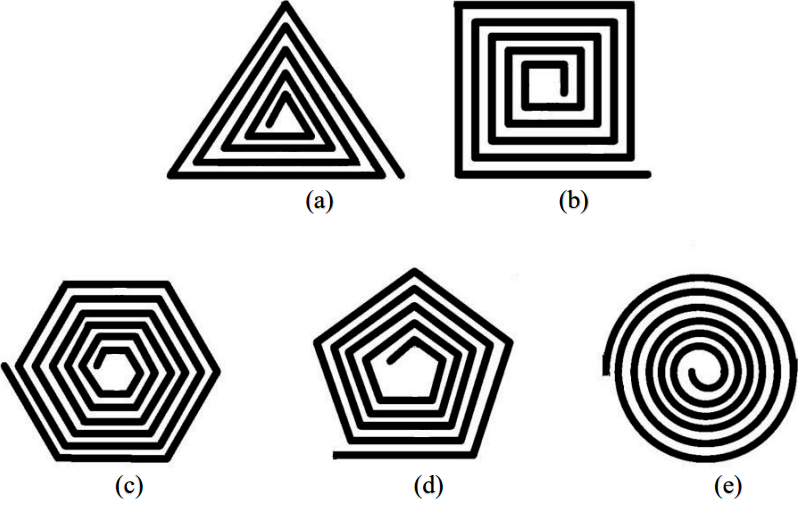
\includegraphics[scale=0.4]{Chapters/Chapter2/PCB_coils/Figures/coils_shapes.png}
    \caption[Coils Shapes]{Different planar coil architectures such as (a) triangle, (b) square, (c)
    pentagon, (d) hexagon, (e) circle.}
    \label{fig: Coils Shapes}
\end{figure}

% -- Subsection 1.2
\subsection{Planar coil magnetic field}
The structure of a planar coil is very different from a standard one, as it is a flat structure with a spiral winding. The magnetic field generated by a planar coil is more complex than that of a standard coil, as the magnetic field is not concentrated in the center of the coil but is distributed over the entire surface of the coil. The magnetic field generated by a planar coil is represented in Figure \ref{fig: Spiral magn field}

\begin{figure}[th]
    \centering
    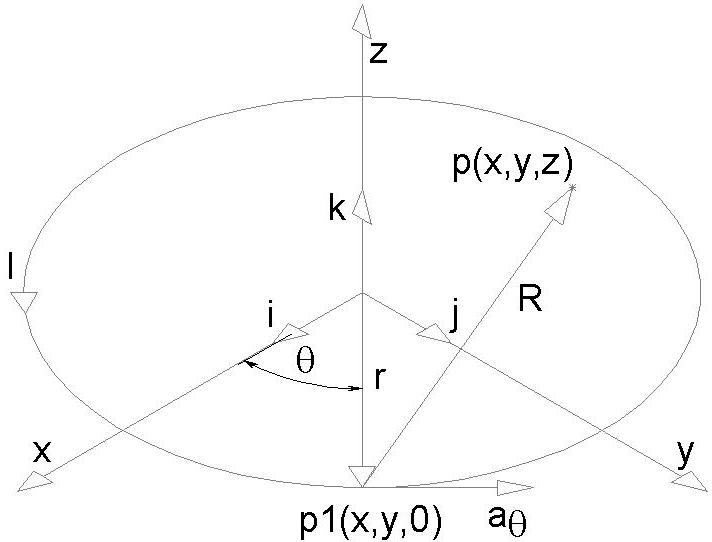
\includegraphics[scale=0.4]{Chapters/Chapter2/PCB_coils/Figures/coil_field_diagram.png} % TODO: Change image with svg
    \caption[Spiral magn field]{(c) Representation of the magnetic field generated by a circular spiral planar coil placed on an aluminum plate.\cite{Spiral_Coil_magn_field}}
    \label{fig: Spiral magn field}
\end{figure}

Then considering again the circular spiral structure, the magnetic field generated by a planar coil at its surface can be derived as

\begin{figure}
    \centering
    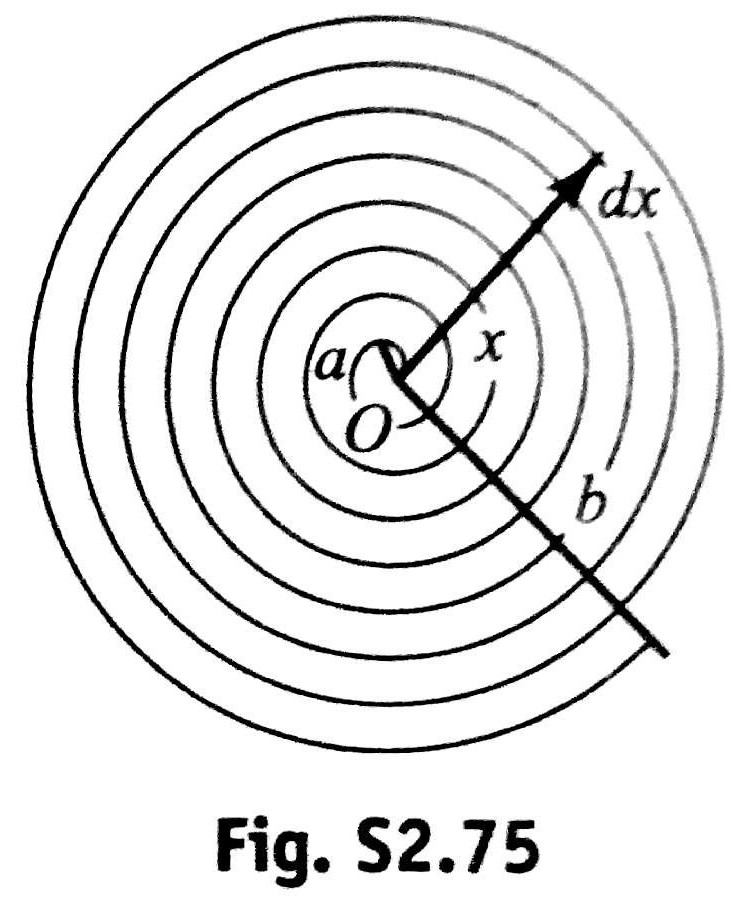
\includegraphics[scale=0.4]{Chapters/Chapter2/PCB_coils/Figures/spiral_windings.jpg} % TODO: Change picture with svg
    \caption[Coil spiral]{Circular spiral coil.}
    \label{fig: Coil spiral}
\end{figure}

\begin{equation}
    Bz = \frac{\mu N I}{2} \cdot \frac{\ln(\frac{b}{a})}{b-a} % https://www.youtube.com/watch?v=1bp9gGCSLc4 TODO: find a reference
    \label{eq: Spiral_magn_field}
\end{equation}

Where:
\begin{itemize}
    \item $Bz$ is the magnetic field on the z-axis [T]
    \item $\mu$ is the magnetic permeability of the medium [H/m]
    \item $n$ is the number of turns of the spiral
    \item $I$ is the current flowing through the wire [A]
    \item $b$ is the external radius of the spiral [m]
    \item $a$ is the internal radius of the spiral [m]
\end{itemize}

To then find the magnetic field at a distance $z$ from the center of the coil, we can use the equation \eqref{eq: Coil_magn_field}from the previous subsection and substitute the radius $r$ of the coil with $r' = \frac{b-a}{\ln(\frac{b}{a})}$  

\begin{equation}
    Bz = \frac{\mu N I r'^2}{2(r'^2+z^2)^\frac{3}{2}}
\end{equation}



% -- Subsection 1.3
\subsection{Multi-layer PCB coils}
Another approach to miniaturizing PCB coils is to create multi-layer coils. 
This is done by stacking multiple layers of PCBs on top of each other, with each layer containing a different part of the coil. This allows for the creation of coils with a higher number of windings in a smaller space. The main challenge with multi-layer PCB coils is the alignment of the different layers. If the layers are not aligned properly, the coil will not function correctly.

Current manufacturing allows for up to 10 layers of PCBs to be stacked on top of each other. However, the more layers that are added, the more difficult it becomes to align the layers correctly.
If the layers are not aligned properly, the magnetic field generated by each layer will also not be aligned, which can lead to a decrease in the efficiency of the coil due to interferences.

\subsubsection{Total inductance}
Considering a two layers coil the total inductance can be calculated as 

\begin{equation}
    L_s = 2L_0 + 2M,   M = K_c \cdot L_0
\end{equation}

Where:
\begin{itemize}
    \item \( L_s \) is the total inductance of the coil [H].
    \item \( L_0 \) is the inductance of a single layer [H].
    \item \( M \) is the mutual inductance between the two layers [H].
    \item \( K_c \) is the coupling coefficient between the two layers.
\end{itemize}

Then $K_c$ can be calculated with an empirical formula derived from multiple measurements by \textit{Jonsenser Zhao} \cite{Multilayer_spiral_inductors} as

\begin{equation}
    K_c = \frac{N^2}{0.64[(0.184d^3-0.525d^2+1.038d+1.001)(1.67N^2-5.84N+65)]}
\end{equation}

Where:
\begin{itemize}
    \item \( N \) is the number of turns of the coil.
    \item \( d \) is the distance between the two layers [m].
\end{itemize}

\subsubsection{Magnetic field generated by a Multilayer coil}
We can use equation \ref{eq:Inductance_&_flux} and $L_s$ calculated in the previous point to find the magnetic flux through the coils
\begin{equation}
    \Phi(I) = L_s \cdot I
\end{equation}

Then with equation \ref{eq:Magnetic_flux_&_field} we can derive the total magnetic field as
\begin{equation}
    B_t = \frac{L_s \cdot I}{\pi r^2}
\end{equation}

Where:
\begin{itemize}
    \item \( B_t \) is the total magnetic field [T].
    \item \( r \) is the radius of the coil [m].
\end{itemize}


% TODO: Maybe insert a graph for the effect of the mutual inductance 




